\chapter{Bound state QED in the Furry picture}
\label{ch:furry_pic}
\begin{itemize}
\item Treatment of perturbations in Furry picture(mixed QED+HFS)
\item Treatment of nuclear structure effects in Furry picture (nuclear excited states)
\item needed notation: sigma, gamma matrices, $\sqrt{p\cdot \sigma}$ in plane wave solutions, $\gamma$, $\alpha$ matrices, def of $a^\mu b_\mu$, def of $x=(x^0,\mathbf{x})$, vector are mathbf, hypergeometric functions

\item conventions for prefactors in lagrangian, def. of gamma matrices: peskin schröder
\item conventions for propagators: itzykson
\item for appendix:  feynman rules (position sp.) qed from itzykson
\end{itemize} 
\section{The external field approximation in QED}
\label{sec:ext_field}
A huge success of the Dirac equation~\cite{dirac1928} was the correct prediction of the fine structure of the hydrogen atom. Originally intended to be a relativistic generalization of the Schrödinger equation, it was a one-particle equation for a classical field. 
However, a relativistic quantum theory always has to be a many-body theory, since for high energies effects like pair creation have to be considered. The relativistic quantum field theory suitable for describing the electromagnetic interaction is quantum electrodynamics (QED). In this framework, the bound state energies of atomic systems can be obtained including radiative corrections due to the quantized photon field and virtual particle-antiparticle pairs. 

In this thesis, hydrogen-like systems and heavy nuclei are considered, so a single fermion (electron or muon) bound to a nucleus with a high charge number $Z$. The interaction strength of electron and nucleus is characterized by the parameter $Z\alpha$, where $\alpha \approx 1/137$ is the fine-structure constant. For high $Z$, this parameter is not small and as a result the Coulomb interaction between fermion and nucleus cannot be treated in perturbation theory. 
For heavy nuclei, the mass ratio $m/M$, where $m$ is the fermion and $M$ is the nuclear mass, is small. Accordingly, the external field approximation ~\cite[\mbox{Section~13.6}]{weinberg2005} $m/M \rightarrow 0$ can be used, which is also called the Furry picture of QED~\cite{furry1951}. Here, recoil effects are neglected and the nucleus is considered as the source of a classical electromagnetic field, which the bound fermion is exposed to.

The basis of the derivations in this chapter is the Lagrangian of QED
\begin{alignat}{6}
\label{eq:Lqed}
\mathcal{L}_{\text{QED}}&=\phantom{:}\bar{\psi}\left( i \gamma^\mu \partial_\mu -m  \right)\psi &&-\frac{1}{4}F_{\mu\nu}F^{\mu\nu}&&-e\bar{\psi}\gamma^\mu \psi A_\mu,\\
&\eqqcolon \mathcal{L}_{\text{free}}^{\text{D}} &&+ \mathcal{L}_{\text{free}}^{\text{E.M.}} &&+ \mathcal{L}_{\text{int}} \nonumber
\end{alignat}
which is the sum of the free Dirac, the free electromagnetic and the interaction Lagrangian. Here, $\psi(x)$ is the fermion field operator, $F_{\mu\nu}=\partial_\mu A_\nu - \partial_\nu A_\mu$ the field strength tensor of the electromagnetic four-potential $A_\mu(x)$. Detailed introductions to QED starting from this Lagrangian can be found in several excellent textbooks, e.g.~\cite{weinberg2005,itzykson2005,peskin1995}, thus the focus of this section is on the external field approximation and extraction of bound state energies. The counter terms are not included, so the derivations here should be understood on a formal level, for calculations including the counterterms and renormalization, see e.g. \cite[Section 14]{weinberg2005}, \cite{shabaev2002_2}.

In the external field approximation, the electromagnetic four-potential is written as
\begin{equation}
A_\mu(x) = \mathcal{A}_\mu(x) + \hat{A}_\mu(x),
\end{equation}
where $\mathcal{A}_\mu(x)$ is the classical four-potential, caused by the nuclear charge and current distribution and $\hat{A}_\mu(x)$ is the quantized field describing quantum fluctuations. Correspondingly, the interaction part in Eq.~\eqref{eq:Lqed} is devided as
\begin{equation}
\label{eq:Lint}
\mathcal{L}_{\text{int}}=-e\bar{\psi}\gamma^\mu \psi \mathcal{A}_\mu-e\bar{\psi}\gamma^\mu \psi \hat{A}_\mu\eqqcolon\mathcal{L}_{\text{int}}^{\text{C}} + \mathcal{L}_{\text{int}}^{\text{Q}}.
\end{equation}
For hydrogen-like systems, bound state energies can be extracted from the poles of the fermion propagator. In the following, it is demonstrated how the poles of the propagator in the interacting theory can be obtained approximately by perturbation theory in powers of the finestructure constant $\alpha$, including the interaction with the classical field to all orders. For this, the full propagator is connected to the propagator in the external classical field and to the propagator of the free theory.
\subsubsection*{Propagator in the free Dirac theory}
As a start, the Lagrangian of the free Dirac theory $\mathcal{L}_{\text{free}}^{\text{D}}$ from Eq.~\eqref{eq:Lqed} is considered. The Euler-Lagrange equations result in the Dirac equation as the equation of motion for the quantum field as
\begin{equation}
\label{eq:dirac}
\left( i\gamma^\mu \partial_\mu -m \right) \psi(x) = 0.
\end{equation}
The solution of Eq.~\eqref{eq:dirac} is written as a superposition of plane-wave solutions~\mbox{\cite[Section~3.3.]{peskin1995}} as
\begin{alignat}{2}
& \psi(x) = 
\int \frac{\mathrm{}d^3p}{(2\pi)^3}\frac{1}{\sqrt{2E_\mathbf{p}}} 
\sum_{s=1}^{2} \left(a^s_\mathbf{p}u^s(p) \e^{-ip\cdot x} + b^{s\,\dagger}_{\mathbf{p}}v^s(p) \e^{ip\cdot x} \right),\\
& \bar{\psi}(x) = 
\int \frac{\mathrm{}d^3p}{(2\pi)^3}\frac{1}{\sqrt{2E_\mathbf{p}}} 
\sum_{s=1}^{2} \left(b^s_\mathbf{p}\bar{v}^s(p) \e^{-ip\cdot x} + a^{s\,\dagger}_{\mathbf{p}}\bar{u}^s(p) \e^{ip\cdot x} \right),\\
\end{alignat}
where the plane wave solutions read as
\begin{alignat}{4}
& u_1(p)= \begin{pmatrix}\sqrt{p\cdot \sigma}\xi_1\\\sqrt{p\cdot \bar{\sigma}}\xi_1\end{pmatrix},\,&& 
u_2(p)= \begin{pmatrix}\sqrt{p\cdot \sigma}\xi_2\\\sqrt{p\cdot \bar{\sigma}}\xi_2\end{pmatrix},\,&& 
v_1(p)= \begin{pmatrix}\phantom{-}\sqrt{p\cdot \sigma}\xi_1\\-\sqrt{p\cdot \bar{\sigma}}\xi_1\end{pmatrix},\,&& 
v_2(p)= \begin{pmatrix}\phantom{-}\sqrt{p\cdot \sigma}\xi_2\\-\sqrt{p\cdot \bar{\sigma}}\xi_2\end{pmatrix}\notag\\
&\text{with}\\
&\xi_1=\begin{pmatrix}1\\0\end{pmatrix},\quad
\xi_2=\begin{pmatrix}0\\1\end{pmatrix}.\notag
\end{alignat}
The Operators $a^{s}_{\mathbf{p}}$, $b^{s}_{\mathbf{p}}$ fulfill the anticommutation relations
\begin{equation}
\left\{ a^{r}_\mathbf{p},a^{s\,\dagger}_\mathbf{q}\right\} = \left\{ b^{r}_\mathbf{p},b^{s\,\dagger}_\mathbf{q}\right\} = (2\pi)^3 \delta (\mathbf{p}-\mathbf{q})\delta_{rs},
\end{equation}
and zero for all other cases. The vacuum state of the theory is defined as the state destroyed by the annihilation operators as
\begin{equation}
a^s_\mathbf{p}\left|0\right> = b^s_\mathbf{p}\left|0\right> = 0,
\end{equation}
while the one-particle fermion and anti-fermion states are created from the vacuum as
\begin{align}
\left|\mathbf{p},s\right> = \sqrt{2E_\mathbf{p}}a^{s\,\dagger}\left|0\right>,\notag\\
\left|\mathbf{q},r\right> = \sqrt{2E_\mathbf{q}}b^{r\,\dagger}\left|0\right>.
\end{align}
Now, the Feynman propagator can be defined as the vacuum expectation value of the time-ordered product~\cite[Section 3.5.]{peskin1995} and reads as
\begin{equation}
S_F(x-y)\coloneqq \left<0\right|T\psi(x)\bar{\psi}(x)\left|0\right>=\int \frac{\mathrm{d}^4p}{(2\pi)^4}\frac{ (\gamma^\mu p_\mu+m)}{p^2-m^2+i\epsilon}\e^{-ip\cdot(x-y)}.
\label{eq:freepropdef}
\end{equation}
The Feynman propagator is a Green's function of the Dirac equation~\eqref{eq:dirac}, thus
\begin{equation}
\left(i\gamma^\mu \partial_\mu -m\right)S_F(x-y)=\delta(x-y)
\label{eq:freeprop}
\end{equation} 
\subsubsection*{Propagator in the external field}
As a next step, we will consider the sum $\mathcal{L}_{\text{free}}^{\text{D}} + \mathcal{L}_{\text{int}}^{\text{C}}$ of free Dirac Lagrangian  and the interaction with the classical external field  from Eq.~\eqref{eq:Lint}. In the following, it is assumed that the external field is independent of time. The equations of motion for the fermion field are
\begin{equation}
\left( i \gamma^\mu \partial_\mu - m - e \gamma^\mu \mathcal{A}_\mu \right)
\psi(x) = 0,
\end{equation}
which simply is the Dirac equation in an external field. However, this is still an equation for the quantum field. The corresponding equation for the classical Dirac field is obtained by using a complete set of states $\left|n\right>$ with energies $E_n$, where $\left|0\right>$ is the vacuum state, and define the Dirac wave functions as matrix elements of the fermion field operator~\mbox{\cite[Section 14.1]{weinberg2005}} as
\begin{alignat}{5}
&u_n(x)&&=&&u_n(\mathbf{x})\,\e^{-iE_nt}&&\coloneqq&&\left<0\right|\psi(x)\left|n\right>\notag\\
&v_n(x)&&=&&v_n(\mathbf{x})\,\e^{+iE_nt}&&\coloneqq&&\left<n\right|\psi(x)\left|0\right>,
\label{eq:wavefct}
\end{alignat}
where the first equality follows from time translation invariance, and is only valid in static background fields. 
Then, it can be shown from the anti-commutation relations of the field operator that the wave functions fulfill the completeness relation
\begin{equation}
\sum_n u_n(\mathbf{x})u_n^\dagger(\mathbf{y}) + \sum_m v_m(\mathbf{x})v_m^\dagger(\mathbf{y})=\delta(\mathbf{x}-\mathbf{y}),
\end{equation}
and that both $u_n(\mathbf{x})$ and $v_n(\mathbf{x})$ satisfy the Dirac equation, now for classical fields:
\begin{alignat}{3}
& \left( i\,\pmb{\alpha} \cdot \mathbf{\nabla} + \beta m + e\, \mathcal{A}^0 - e\, \pmb{\alpha}\cdot \pmb{\mathcal{A}} \right) u_n(\mathbf{x}) &&=&& \phantom{-}\;\, E_n u_n(\mathbf{x}) \notag\\
& \left( i\,\pmb{\alpha} \cdot \mathbf{\nabla} + \beta m + e\, \mathcal{A}^0 - e\, \pmb{\alpha}\cdot \pmb{\mathcal{A}} \right) v_n(\mathbf{x}) &&=&& -E_n v_n(\mathbf{x})
\label{eq:diraceq}
\end{alignat}
The Propagator in the external field is defined, similar to Eq.~\eqref{eq:freepropdef}, as the vacuum expectation value of time-ordered product
\begin{equation}
S_{\mathcal{A}}(x,y):=\left<0_\mathcal{A}\right|T\psi(x)\bar{\psi}(x) \left|0_\mathcal{A}\right>,
\label{eq:extpropdef}
\end{equation}
where $\left|0_\mathcal{A}\right>$ denotes the vacuum state in the external field.
It is a Green's function of the equation of motion of the fermion field operator, analogously to Eq.~\eqref{eq:freeprop}:
\begin{equation}
\left(i\gamma^\mu \partial_\mu -m - e \gamma^\mu A_\mu\right)S_{\mathcal{A}}(x,y)=\delta(x-y)
\label{eq:extprop}
\end{equation}
Since the external field violates translation invariance, the propagator in the external field no depends on $x$ and $y$ separately, and not only on the difference $x-y$. Radiative corrections in the Furry picture can be calculated by using the usual Feynman rules and using the dressed propagator instead of the free propagator as well as solutions of the Dirac equation including the external field for the in and out states. Combining Eq.~\eqref{eq:freeprop} with Eq.~\eqref{eq:extprop} gives a relation between the propagators of the free theory and in the external field~\mbox{\cite[Section 2.5.]{itzykson2005}}, which can be solved iteratively, as
\begin{alignat}{2}
&\,S_{\mathcal{A}}(x,y)&&= \,S_F(x-y) 
+ \int\mathrm{d}x\, \,S_F(x-z)\left(-e\gamma^\mu A_\mu(z)\right)\,S_{\mathcal{A}}(z,y)\\
& &&=\,S_F(x-y)+\int\mathrm{d}z\,\,S_F(x-z)(-e\gamma^\mu A_\mu(z))\,S_F(z-y)\\
&&&\phantom{=}+\iint\mathrm{d}z_1\mathrm{d}z_2\,\,S_F(x-z_1)(-e\gamma^\mu A_\mu(z_1))\,S_F(z_1-z_2)(-e\gamma^\mu A_\mu(z_2))\,S_F(z_2-y)\\
&&&\phantom{=}+...\,\,.\label{eq:propeq}
\end{alignat}
As demonstrated in Fig.~\ref{fig:propagator}, this gives an intuitive picture of the dressed propagator: Propagation in the external field corresponds to free propagation with all possible interactions with the external field included.
%
\begin{figure}%
\centering
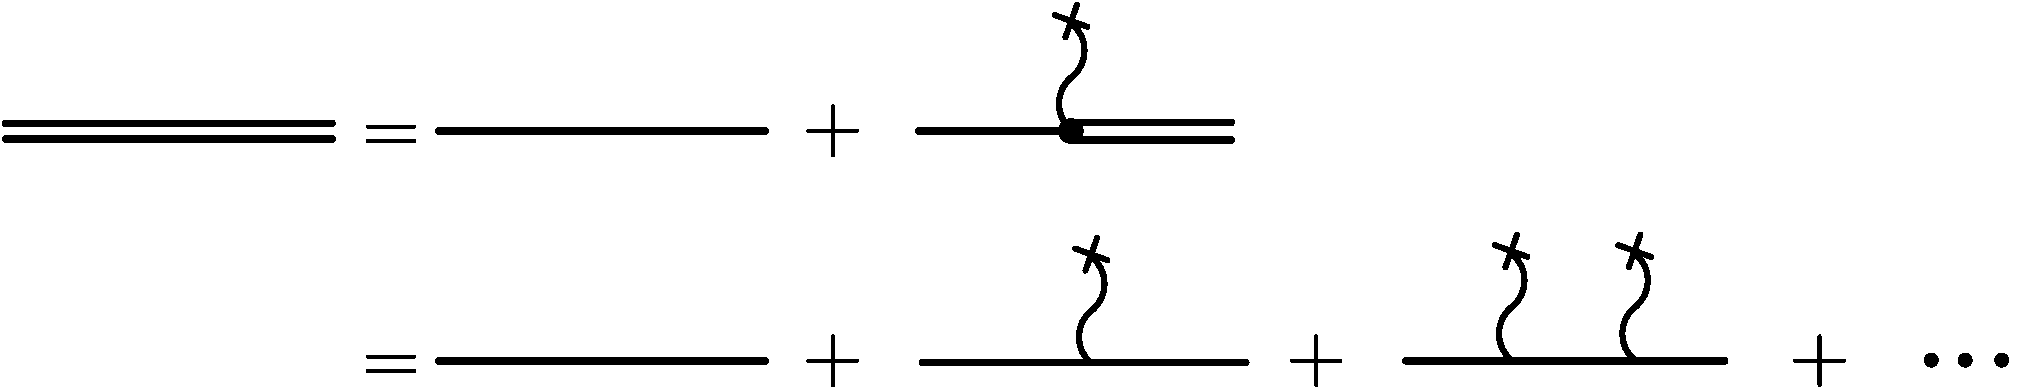
\includegraphics[width=0.9\linewidth]{pics/propagator.pdf}%
\caption{Relation between the propagator including the external field and the propagator of the free theory in Feynman diagrams corresponding to Eq.~\eqref{eq:propeq}. A double line corresponds to the dressed propagator in the external field, a single line to the free Dirac propagator, and a wave line with a cross to the interaction with the external field. The propagator in the external field is obtained by including all interactions with the external field in the free propagator.}%
\label{fig:propagator}%
\end{figure}
%
Another useful form of the Propagator in the external field is the spectral representation in terms of the Dirac wave functions~\eqref{eq:wavefct}. By inserting a complete set of states in Eq.~\eqref{eq:extpropdef}, one obtains
\begin{equation}
S_\mathcal{A}(x,y)=\Theta(x^0-y^0) \sum_n u_n(x)\bar{u}_n(y)
-\Theta(y^0-x^0)\sum_m v_m(x)\bar{v}_m(y).
\end{equation}
For a time-independent external field, a Fourier transformation in the zeroth component yields
\begin{equation}
\tilde{S}(\mathbf{x},\mathbf{y},E)= \sum_n \frac{u_n(\mathbf{x})\bar{u}_n(\mathbf{y})}{E_n -E -i\,\epsilon}
+\sum_m \frac{v_m(\mathbf{x})\bar{v}_m(\mathbf{y})}{E_m +E -i\,\epsilon}.
\label{eq:spectralrep}
\end{equation}
Therefore, bound states due to the external field lead to additional isolated poles in the propagator.

\subsubsection*{Propagator of interacting theory}
Finally, we will consider the propagator in the interacting theory, including the interaction with the quantized photon field. A similar argument as in the derivation of Eq.~\eqref{eq:spectralrep} also holds for the interacting theory~\cite[Section 14.2.]{weinberg2005}. This is, bound state energies including all radiative corrections appear as isolated poles of the full propagator. In order to locate the positions of these poles, perturbation theory with the propagator including the external field is used, expanding the propagator in powers of the finestructure constant $\alpha=e^2/(4\pi)$. The zero-order term is the dressed propagator in the background field, corresponding to solving the Dirac equation with the background field. The diagrams contributing to the radiative corrections to first order in $\alpha$ are the vacuum-polarization~(VP) and self-energy~(SE) diagrams shown in Fig.~\ref{fig:1loop} $(a)$ and $(b)$, respectively. Using the Feynman rules~\mbox{\cite[Section 6.1.]{itzykson2005}}, the propagator of the interacting theory $S_{I}(x,y)$ is expanded to first order in $\alpha$ as
\begin{alignat}{2}
&S_{I}(x,y) &&\approx S_{\mathcal{A}}(x,y) + \int \mathrm{d}^4z_1\,\mathrm{d}^4z_2\,
S_{\mathcal{A}}(x,z_1)\,\left[\Sigma_{\text{VP}}(z_1,z_2)+\Sigma_{\text{SE}}(z_1,z_2)\right]\,S_{\mathcal{A}}(z_2,y),\notag\\
&\text{with }\notag\\
&\Sigma_{\text{VP}}(z_1,z_2)&&\coloneqq-\delta(z_1-z_2)(-ie\gamma^\mu)\int \text{d}z\,S_P(z_1-z)\Tr ((-ie\gamma_\mu)S_{\mathcal{A}}(z,z)),\notag\\
&\Sigma_{\text{SE}}(z_1,z_2)&&\coloneqq(-ie\gamma^\mu)S_{\mathcal{A}}(z_1,z_2)S_P(z_1-z_2)(-ie\gamma_\mu),
\end{alignat}
where $g_{\mu\nu}S_P(x-y)$ is the photon propagator in position space~\mbox{\cite[Section 3.2.]{itzykson2005}}. Using the Fourier transformed functions
\begin{equation}
\Sigma_{\text{VP/SE}}(\mathbf{z}_1,\mathbf{z}_2,E)= \int \text{d}z_1^0\, \e^{iE(z_1^0-z_2^0)}\Sigma_{\text{VP/SE}}(z_1,z_2),
\end{equation}
and the spectral representation of the propagator from Eq.~\eqref{eq:spectralrep}, the levelshifts of the $n$-th level can be extracted from the shift of the poles~\mbox{\cite[Section 14.2.]{weinberg2005}} as
\begin{equation}
\Delta E_n = \int \text{d}^3\mathbf{x}\,\text{d}^3\mathbf{y}\,\bar{u}_n(\mathbf{x})\left( -\Sigma_{\text{VP}}(\mathbf{x},\mathbf{y},E_N)-\Sigma_{\text{SE}}(\mathbf{x},\mathbf{y},E_N) \right)u_N(\mathbf{y}).
\end{equation}
%
\begin{figure}%
\centering
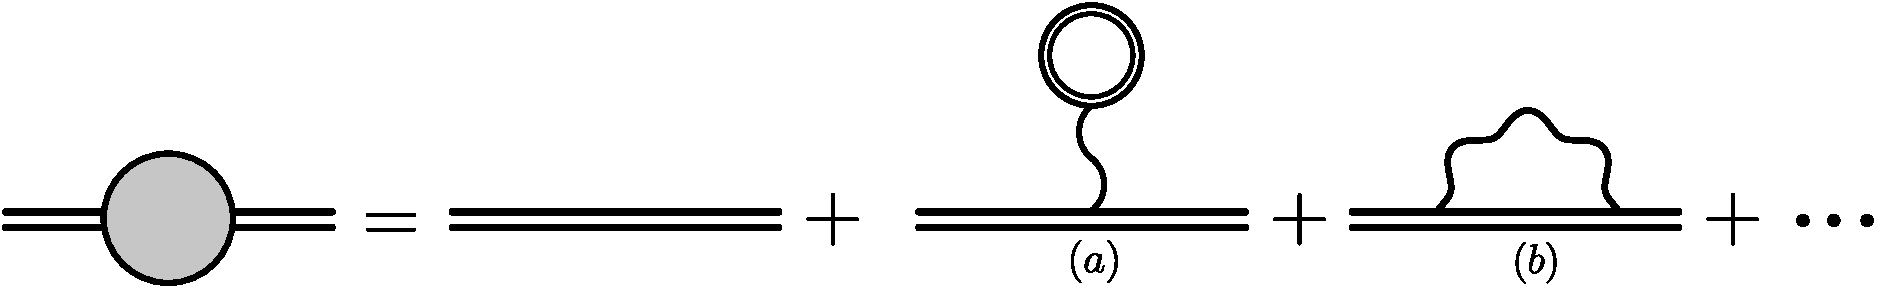
\includegraphics[width=0.9\linewidth]{pics/1loop.pdf}%
\caption{Perturbative expansion of the propagator of the interacting theory in powers of~$e^2$. The zero-order contribution is the propagator in the external field. To first order in~$e^2$, the contributions are the vacuum-polarization diagramm~$(a)$ and the self-energy diagram~$(b)$.}%
\label{fig:1loop}%
\end{figure}
%

\subsection{Vacuum polarization potentials}
For practical calculations of the order $\alpha$ vacuum polarization, the closed fermion loop in Fig.~\ref{fig:1loop}~b) can be expanded in numbers of interactions with the background field, using Eq.~\ref{eq:propeq}. For the case of atomic physics, since the nuclear potential is proportional to the nuclear charge number $Z$, this expansion is in powers of $Z\alpha$. The corresponding diagrams in order $\alpha(Z\alpha)$ (Uehling potential~\cite{uehling1935}) and $\alpha(Z\alpha)^3$ (Wichmann-Kroll potential~\cite{wichmann1956}) are shown in Fig.~\ref{fig:vac_pol_wk}. Since the closed loop now is formed by the free fermion propagator, all diagramms of order $\alpha(Z\alpha)^n$ with even $n$ vanish as a consequence of Furry's theorem~\mbox{\cite[Section~10.1.]{peskin1995}}. Formally, the order $\alpha (Z\alpha)$ correction $\delta S_{\text{Uehl}}$ from diagram (a) in Fig.~\ref{fig:vac_pol_uehl} to the propagator $S_{\mathcal{A}}$ reads
\begin{alignat}{3}
\label{eq:uehl}
&\delta S_{\text{Uehl}}(x,y) &&=&& \int \mathrm{d}z_1\,S_{\mathcal{A}}(x,z_1)\Sigma_{\text{Uehl}}(z_1)S_{\mathcal{A}}(z_1,y)\\
&\text{with}\notag\\
&\Sigma_{\text{Uehl}}(z_1) &&\coloneqq&& -\int\mathrm{d}z_2(-ie\gamma^\mu)S_P(z_1-z_2)\notag\\
&&&&&\times\int\mathrm{d}z_3\,\Tr((-ie\gamma_\mu)S_F(z_2-z_3)(-e\gamma^\nu A_\nu (z_3))S_F(z_3-z_2)).\notag
\end{alignat}
Analogously to the inclusion of the external field in the propagator from Eq.~\eqref{eq:extprop}, Eq.~\eqref{eq:uehl} and the corresponding iterations from diagrams (b), (c),$\,$... in Fig.~\ref{fig:vac_pol_uehl} can be summed to define a propagator $S_{\mathcal{A}+\text{Uehl}}$ which contains all iterations both in the external field and the order $\alpha (Z\alpha)$ vacuum polarization via the integral equation
\begin{equation}
S_{\mathcal{A}+\text{Uehl}}(x,y) = S_{\mathcal{A}}(x,y) +  \int \mathrm{d}z_1\,S_{\mathcal{A}}(x,z_1)\Sigma_{\text{Uehl}}(z_1)S_{\mathcal{A}+\text{Uehl}}(z_1,y).
\label{eq:uehlsum}
\end{equation}
This propagator is a Green's function for the Dirac equation including the external field and the Uehling potential as
\begin{equation}
\left(i\gamma^\mu \partial_\mu -m - e \gamma^\mu A_\mu + \Sigma_{\text{Uehl}}\right)S_{\mathcal{A}+\text{Uehl}}(x,y)=\delta(x-y).
\label{eq:uehlprop}
\end{equation}
As a result, the diagrams in Fig.~\ref{fig:vac_pol_uehl} can be calculated by solving the Dirac equation~\eqref{eq:diraceq} including the Uehling potential. The same reasoning holds as well for the Wichmann-Kroll potential (Fig.~\ref{fig:vac_pol_wk}~b)) and for the order $\alpha^2(Z\alpha)$ vacuum polarization, referred to as the Källen-Sabry potential~\cite{kallen1955}, where the corresponding diagrams are shown in Fig.~\ref{fig:vac_pol_ks}. 

Since the formal expressions for the vacuum polarization potentials contain divergences, they have to be renormalised. The corresponding expressions for the renormalized Uehling, Wichmann-Kroll and Källen-Sabry potentials are given in Section~\ref{sec:sph_dirac}.
%
\begin{figure}%
\centering
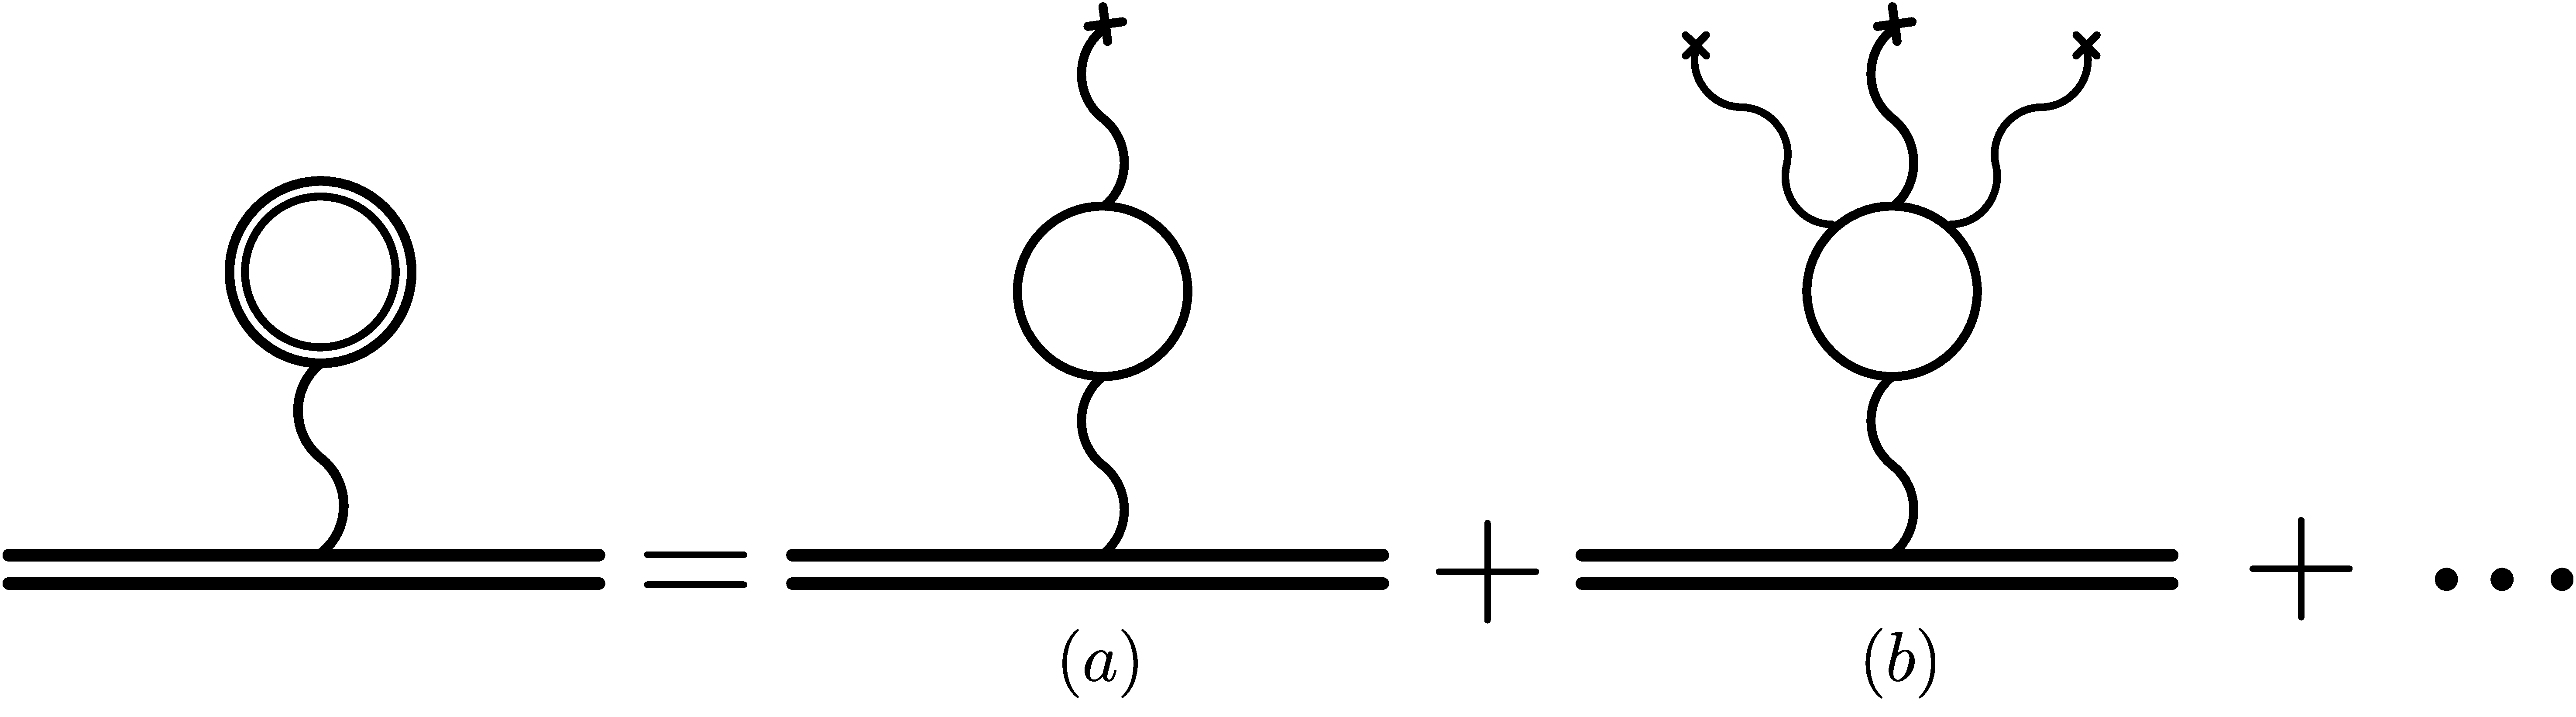
\includegraphics[width=0.75\linewidth]{pics/vac_pol_wk.pdf}%
\caption{Expansion of the order $\alpha$ vacuum polarization in powers of $(Z\alpha)$, i.e. in number of interactions with the nuclear field. The contributions with odd powers vanish due to Furry's theorem. The $\alpha(Z\alpha)$ contribution (diagram $a$) is the Uehling term, the $\alpha(Z\alpha)^3$ contribution (diagram $b$) is the Wichmann-Kroll term.}%
\label{fig:vac_pol_wk}%
\end{figure}
%
%
\begin{figure}%
\centering
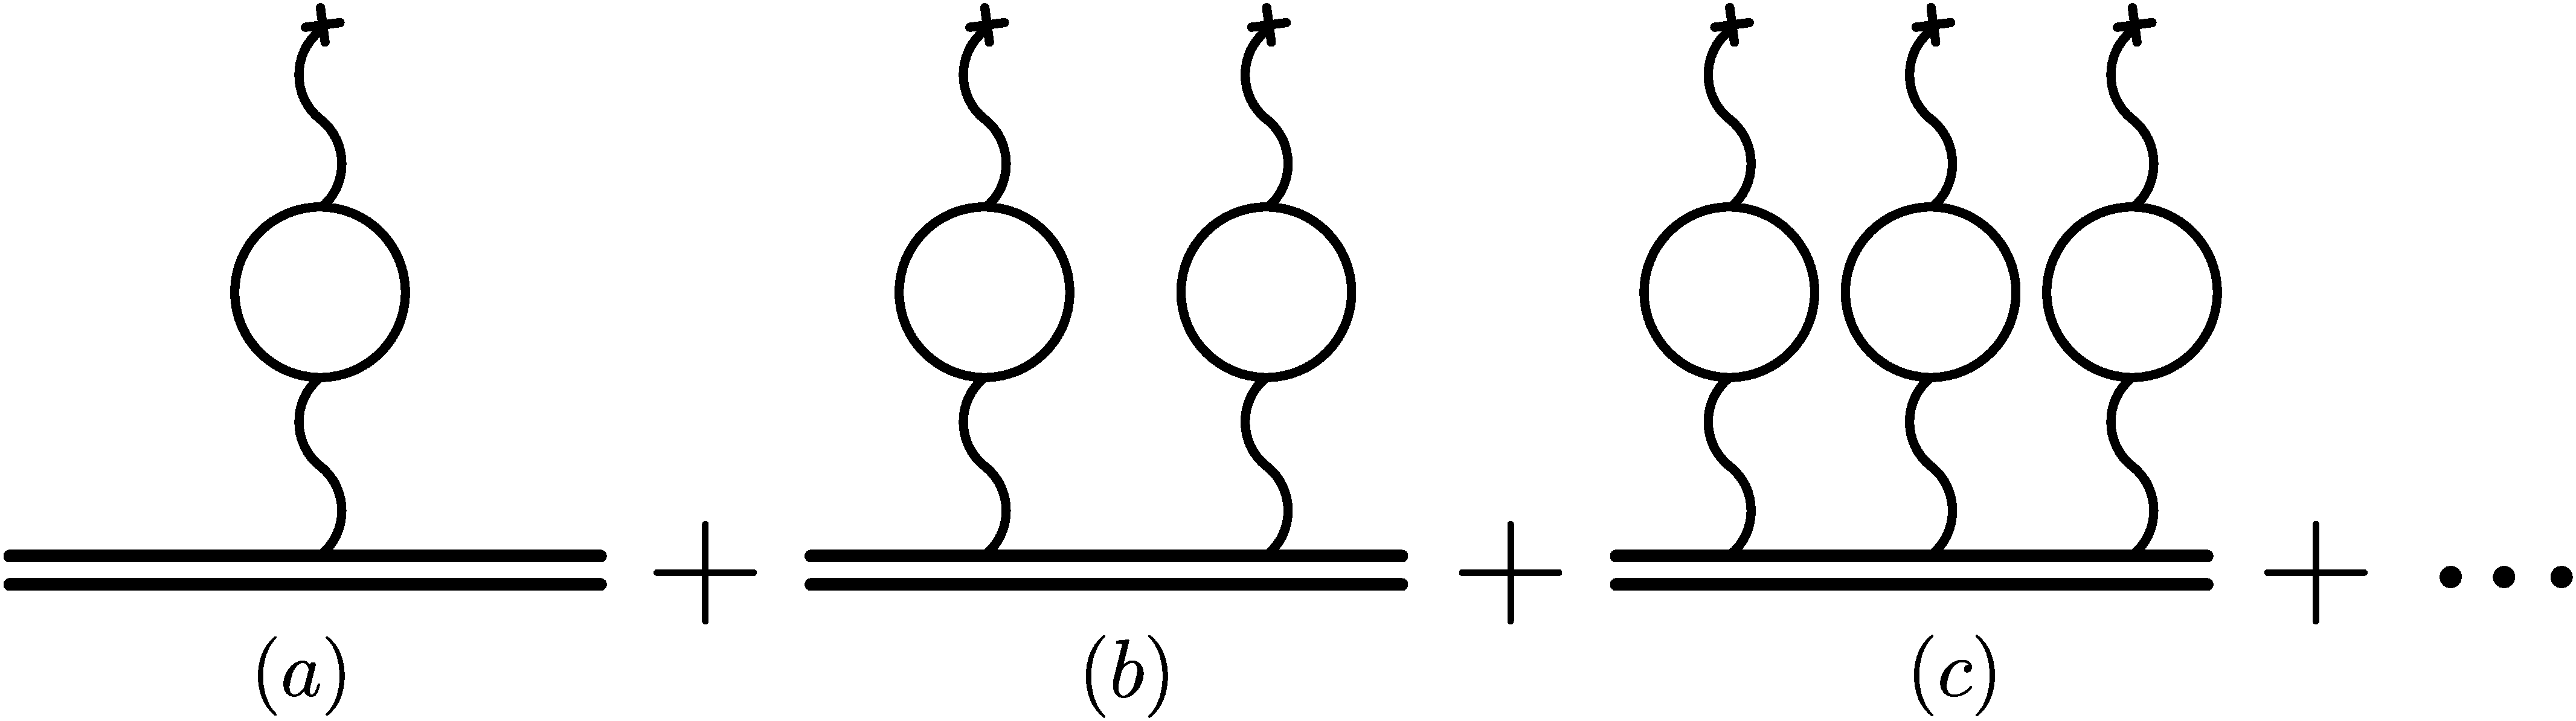
\includegraphics[width=0.8\linewidth]{pics/vac_pol_uehl.pdf}%
\caption{Resummation of iterations of the Uehling potential needed for the modified Propagator from Eq.~\eqref{eq:uehlsum}.}%
\label{fig:vac_pol_uehl}%
\end{figure}
%
%
\begin{figure}%
\centering
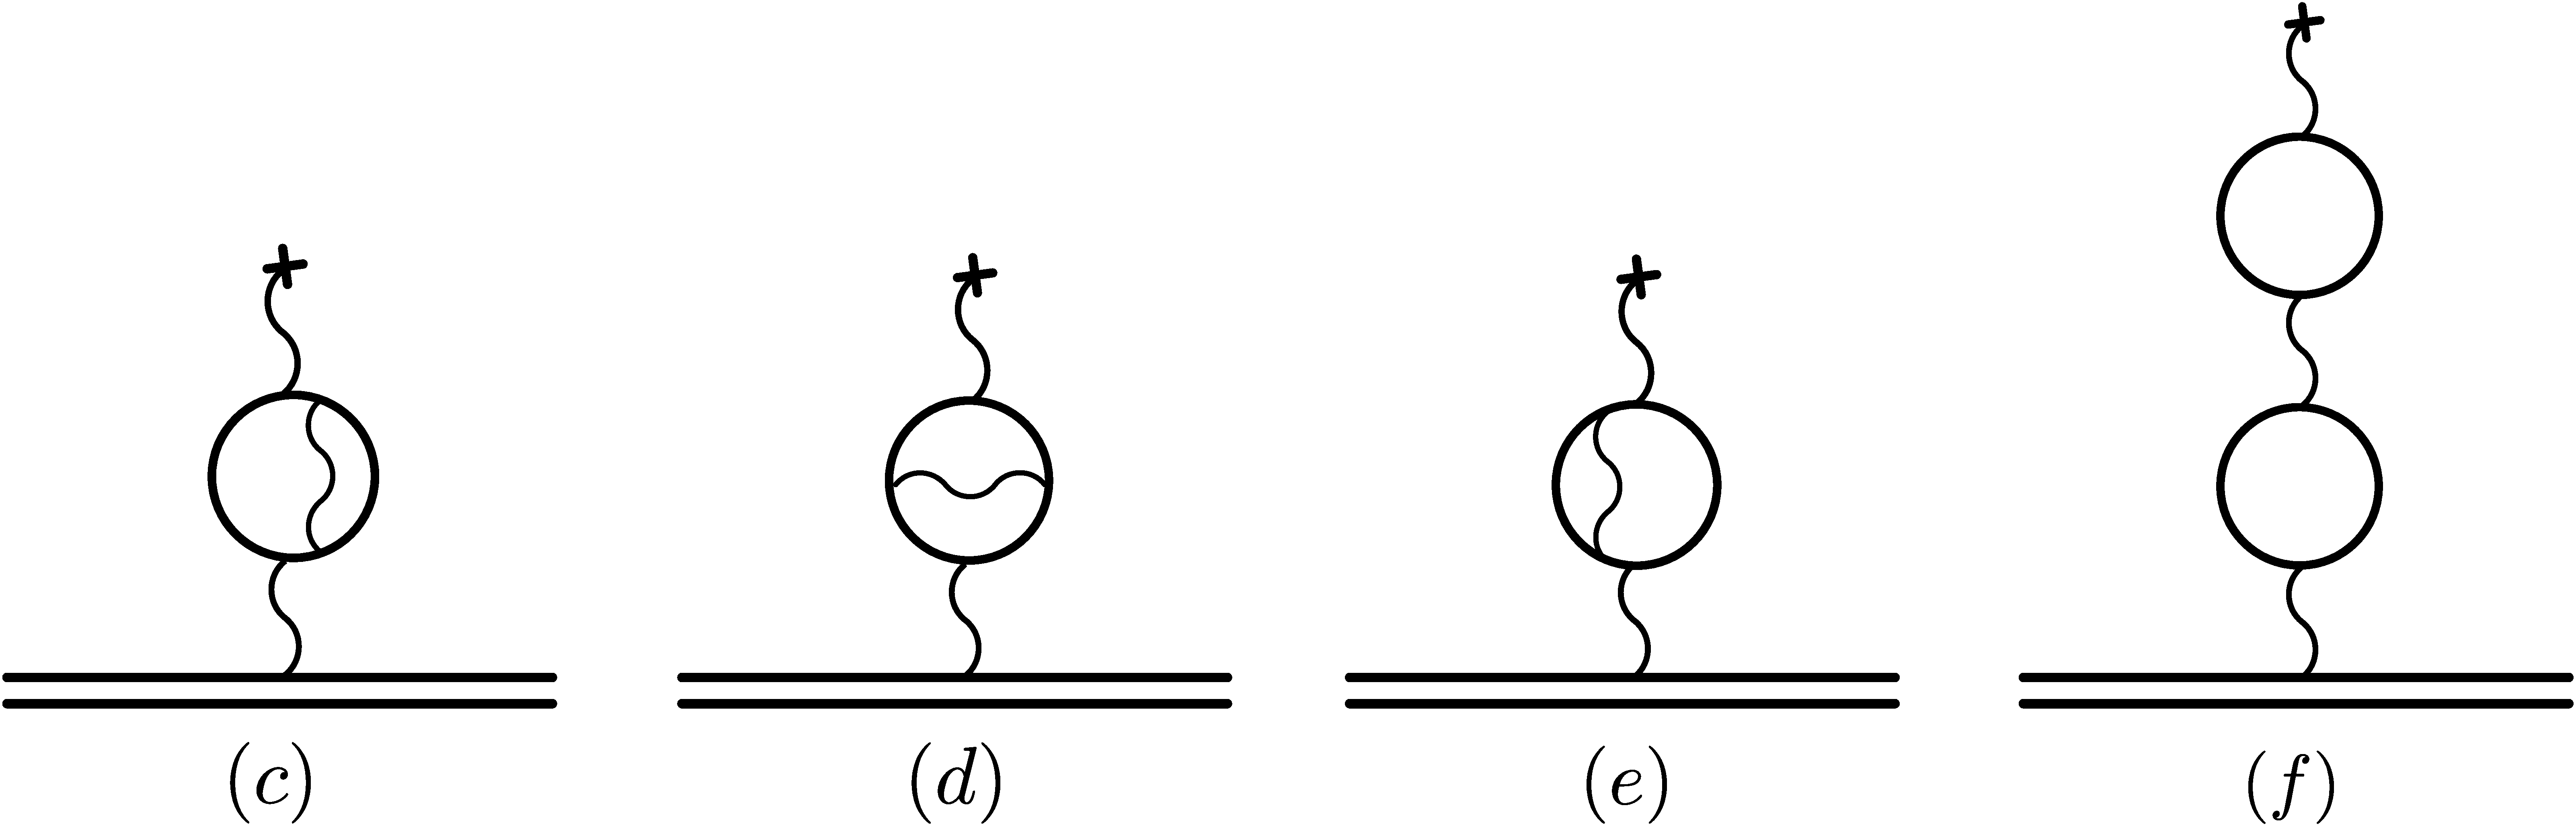
\includegraphics[width=0.9\linewidth]{pics/vac_pol_ks.pdf}%
\caption{Feynman diagrams corresponding to the contributions to the Källen-Sabry potential of order $\alpha^2(Z\alpha)$.}%
\label{fig:vac_pol_ks}%
\end{figure}
%
\section{Dirac equation in central potentials}
\label{sec:sph_dirac}
In the previous Section, the binding energies of a fermion bound by an atomic nucleus were investigated in the framework of the Furry picture of QED. The zeroth order approximations turned out to be the eigenenergies of the solutions of the Dirac equation (for a c-number field) including the nuclear background field. Furthermore, it was demonstrated that certain radiative corrections can be included as potentials in the Dirac equation as well. To a first approximation, the nuclear potential can be described by a static electric field which possesses spherical symmetry, and deviations thereof may be treated by perturbation theory later on. Thus, in this Section, the solutions of the Dirac equation for a spherical symmetric potential are discussed, mainly following~\cite{greiner2000, weinberg2005}. Then, the case of the pure Coulomb potential is discussed, where the solution can be given in closed form due to the high degree of symmetry. Finally, the dual-kinetic-balance method~\cite{Shabaev2004} for obtaining numerical solutions for arbitrary spherical symmetric potentials is discussed.

Firstly, the Dirac equation~\eqref{eq:diraceq} for the functions $v_n$ is rewritten, such that it has the same form as for $u_n$. For this, add a new range of indices $\tilde{n}$ to the original $n$ and define $u_{\tilde{n}}(x)\coloneqq v_n(x)$, $E_{\tilde{n}}\coloneqq -E_n$. Secondly, static electric background fields are considered, which corresponds to a four potential
\begin{equation}
\mathcal{A}_\mu(x)=(\Phi(\mathbf{x})/e,\mathbf{0}),
\end{equation}
where the electric potential $\phi(\mathbf{r})$ can be expressed in terms of a spherically symmetric nuclear charge distribution $\rho(\mathbf{|r|})$ as
\begin{equation}
\label{eq:furry_elPot}
\Phi(\mathbf{r})=-Z\alpha\int\mathrm{d}V^{\prime}\,\frac{\rho(|\mathbf{r^{\prime}}|)}{|\mathbf{r}-\mathbf{r^{\prime}}|},
\end{equation}
where $\int \mathrm{d}V\,\rho(|\mathbf{r}|)=1$. Since $\Phi$ only depends on $|\mathbf{r}|$, we define $V(r)\coloneqq \Phi((r,0,0))$ for spherical coordinates $\mathbf{r}=(r,\vartheta,\varphi)$. Thereby, the Dirac equation~\eqref{eq:diraceq} reads as
\begin{equation}
\text{H}_D \, u_n(\mathbf{r})\coloneqq\left( i\,\pmb{\alpha} \cdot \mathbf{\nabla} + \beta m + V(r) \right) u_n(\mathbf{r}) =  E_n u_n(\mathbf{r}),
\label{eq:sphdirac}
\end{equation}
where the eigenenergies $E_n$ contain both positive and negative values and the spectrum contains both continuum and discrete parts. $u_n(\mathbf{r})$ are the corresponding solutions in form of four-component spinors. For an arbitrary potential $V(r)$ possessing spherical symmetry, the solution can be simplified significantly by transforming the partial differential equation~\eqref{eq:sphdirac} into an ordinary differential equation.

For the Dirac Hamiltonian with spherically symmetry, energy eigenfunctions can be found, which also have a well-defined Parity and total angular momentum. At first, the relativistic angular momentum number $\kappa$ is introduced as a function of the orbital angular momentum quantum number $l$ and total angular momentum quantum number $j$ as
\begin{equation}
\kappa(j,l) \coloneqq (-1)^{j+l+1/2} \left(j+\frac{1}{2}\right).
\end{equation}
Since for a Dirac particle every value of $l$ has two possible values $j=l\pm 1/2$, the mapping $\kappa \leftrightarrow (j,l)$ is bijective with $j(\kappa)=|\kappa|-1/2$; $l(\kappa)=|\kappa|+(\mathrm{sgn}(\kappa)-1)/2$. Eigenfunctions of the total angular momentum can be constructed by the eigenfunctions of the orbital angular momentum and spin operator, the spherical harmonics $\text{Y}_{lm}(\vartheta,\varphi)$ and two-component spinors $\chi_{\nicefrac{1}{2}}=(1,0)^T$; $\chi_{\nicefrac{-1}{2}}=(0,1)^T$, respectively as
\begin{equation}
\Omega_{\kappa m}(\vartheta,\varphi)\coloneqq
\sum_{{\scriptscriptstyle {m_l}{=}{-l(\kappa)}}}^{\scriptscriptstyle l(\kappa)}\;
\sum_{{\scriptscriptstyle {m_s}{=}{\nicefrac{-1}{2}}}}^{\scriptscriptstyle \nicefrac{1}{2}}
\text{C}^{j(\kappa)m}_{l(\kappa)m_l\,\nicefrac{1}{2}\,m_s}
\text{Y}_{l(\kappa)m_l}(\vartheta,\varphi)\chi_{m_s},
\label{eq:sph_spinor}
\end{equation}
where $\text{C}^{l_1m_1}_{l_2m_2\,l_3m_3}$ are the Clebsch-Gordan coefficients~\cite{varshalovich1988}. The functions defined in Eq.~\eqref{eq:sph_spinor} are called \textit{spherical spinors}. Direct calculations shows that a pair ($\Omega_{\kappa m}$, $\Omega_{-\kappa m}$) have the same values for $j$, but opposite parity. Motivated by the solutions of the free Dirac equation, the solution is written with an ansatz in two component spinors, with a priori different values for $\kappa_1$, $\kappa_2$, $m_1$, $m_2$. 
However, for a well defined total angular momentum and $z$-component of the total angular momentum $|\kappa_1|=|\kappa_2|$ and $m_1=m_2$ is needed. Furthermore, applying the parity operator reveals that the lower component needs to have the opposite parity compared to the upper component in order for the four-component spinor having a well-defined parity, which corresponds to the parity of the upper component, and therefore $\kappa_1=-\kappa_2$. As a result, the solutions are written as
\begin{equation}
u_{n\kappa m_j}(\mathbf{r})=
\begin{pmatrix}
g_{n\kappa}(r)\Omega_{\kappa m_j}(\vartheta,\varphi)\\
i f_{n\kappa}(r) \Omega_{-\kappa m_j}(\vartheta,\varphi)
\end{pmatrix}.
\label{eq:ansatz_dirac}
\end{equation}
Using this ansatz in the Dirac equation~\ref{eq:sphdirac} leads to the following system of equations for the radial functions $g_{n\kappa}(r)$ and $f_{n\kappa}(r)$:
\begin{numcases}{}
\label{eq:radial_equations_small}
 \frac{\mathrm{d}g(r)}{\mathrm{d}r}+(1+\kappa)\frac{g(r)}{r}
-\left[ E+m-V(r) \right] f(r) = 0\\
\frac{\mathrm{d}f(r)}{\mathrm{d}r}+(1-\kappa)\frac{f(r)}{r}
+\left[ E-m-V(r) \right] g(r) = 0.\notag
\end{numcases}

\subsection{Bound state solutions of the Coulomb problem}
For a point-like nucleus with charge number $Z$, the pure Coulomb potential reads
\begin{equation}
V_C(r)=-\frac{Z\alpha}{r},
\end{equation}
and the radial equations~\eqref{eq:radial_equations_small} can be solved analytically in this case. As a first step, the radial wave functions are substituted with
\begin{alignat}{2}
&g_{n\kappa}(r)&&= \sqrt{1+E_{n\kappa}}\e^{-\lambda r}(\varphi_1(r)+\varphi_2(r)) \\
&f_{n\kappa}(r)&&=\sqrt{1-E_{n\kappa}}\e^{-\lambda r}(\varphi_1(r)-\varphi_2(r)),
\end{alignat}
and for the functions $\varphi_i(r)$ the power-series ansatz
\begin{equation}
\varphi_i(r)=(2\lambda r)^\gamma \sum_{m=0}^\infty a^{(i)}_m (2\lambda r)^m,
\end{equation}
is assumed, where $\lambda = \sqrt{1-E^2_{n\kappa}}$ and $\gamma=\pm \sqrt{\kappa^2 - (Z\alpha)^2}$. Plugging this ansatz in the radial equations~\eqref{eq:radial_equations_small} results in recurrence relations, such that the solution can be expressed only in terms of the normalization coefficient $a^{(1)}_0$ as
\begin{alignat}{2}
& \varphi_1(r)&&=a^{(1)}_0 (2\lambda r)^\gamma\, \text{F}(1-n_r,2\gamma+1,2\lambda r)\\
& \varphi_2(r) &&= a^{(1)}_0 (\kappa -Z\alpha / \lambda) (2\lambda r)^\gamma\, \text{F}(-n_r,2\gamma+1,x) /n_r,
\end{alignat}
where $n_r=Z\alpha E_{n\kappa}/\lambda - \gamma$ and $\text{F}(a,b,c)$ are the confluent hypergeometric function. Now, for the positive value of $\gamma$, the solutions are regular at the origin, but behave as $\e^{\lambda r}$ as $r\rightarrow \infty$. On the other hand, linear combination of positive and negative values of $\gamma$ enable solutions which are regular at infinity but behave badly at the origin. Solutions regular both at the origin and at infinity can only be obtained for certain energies, corresponding to integer values of $n_r$~\cite{rose1961}. With $n=n_r+|\kappa|$, the bound state energies read
\begin{equation}
\label{eq:finestructure_formula}
E_{n\kappa}=\cfrac{(mc^2)}{\sqrt{1+\cfrac{(Z\alpha)^2}{\left( n-|\kappa|+\sqrt{|\kappa|^2-(Z\alpha)^2} \right)^2}}},
\end{equation}
for $n\in \{1,2,3,...\}$ and $0\neq \kappa \in \{{-}{n},...,n-1\}$.
These solution explains the spectrum of hydrogen-like atoms to a reasonable accuracy, including fine structure splitting, as long as $Z\alpha\ll 1$. The solutions are degenerate in the sign of $\kappa$, i.e. states with the same $j$ but different $l$ have the same energy. As a result, the $2s\nicefrac{1}{2}$ and $2p\nicefrac{1}{2}$ states are degenerate. The lifting of this degeneracy (Lamb shift) is explained by radiative corrections and finite nuclear size effects. However, in situations where $Z\alpha$ is not much smaller than unity, the point-like approximation becomes increasingly worse and solutions of the Dirac equation for non-Coulomb potentials have to be used.



\subsection{Numerical solution in a cavity for arbitrary potentials}
Except the rare cases, where the radial equations~\eqref{eq:radial_equations_small} can be solved exactly (eg. Coulomb potential, spherical potential well), numerical methods have to be used to obtain approximations for $g(r)$ and $f(r)$. Especially for atomic systems with large finite nuclear size effects, like highly charged, heavy ions and heavy muonic atoms, the nuclear potential deviates from the Coulomb potential significantly and numerical solutions have to be found, including the extended nuclear charge distribution.
 
Generally, for finite basis set solutions of the Dirac equation, the radial equations~\eqref{eq:radial_equations_small} are considered, but the domain is changed from $r\in[0,\infty)$ to a finite cavity $r\in [0,R]$. On the original domain, the spectrum of the energy eigenvalues $E$ has a negative continuum $E\in (-\infty,-m]$, a positive continuum $E\in [m,\infty)$, and a discrete part $E\in (-m,m)$ of infinitely many bound states, where $m$ is the mass of the bound fermion. On the modified domain, the positive and negative continuum become discrete~\cite{johnson1988}, but still infinite.
A problem with numerical solutions of the Dirac equation is the appearance of unphysical, or spurious states~\cite{johnson1988, drake1981}. A method circumventing this problem was presented in~\cite{Shabaev2004}, which is shortly described in the following.

The radial equations~\eqref{eq:radial_equations_small} can be rewritten in matrix form as
\begin{equation}
\begin{pmatrix}
m+V(r)&(-\partial_r + \kappa/r)\\
(\partial_r + \kappa/r)&-m+V(r)
\end{pmatrix}
\nu(r)\eqqcolon\mathrm{H}_\kappa \nu(r)
= E\,\nu(r)
\label{eq:radmatrixEq}
\end{equation}
for the function $\nu(r)=(G(r),F(r))^T=(r g(r),r f(r))^T$. As a finite set of basis functions, B-splines $\Pi_{i,k}(r)$ of order $k$  with a suitable knot sequence as described in~\cite{johnson1988} are selected, where the first and last spline is set to zero. With the size of the basis set $n$, the solutions are expressed with $2n$ coefficients $c_i$ as
\begin{equation}
\nu(r)=\hspace{-0.2cm}\sum_{i=1}^{2n}c_i\,\nu_i(r)\coloneqq \hspace{-0.2cm}\sum_{i=1}^n
c_i\begin{pmatrix}
\Pi_{i,k}(r)\\
(\partial_r +\kappa/r)\Pi_{i,k}(r)/(2m).
\end{pmatrix}
+\hspace{-0.3cm}
\sum_{i=n+1}^{2n}c_i
\begin{pmatrix}
(\partial_r -\kappa/r)\Pi_{i,k}(r)/(2m)\\
\Pi_{i,k}(r)
\end{pmatrix}\hspace{-0.1cm}.
\label{eq:finitebasis}
\end{equation}
Thereby, the infinite amount of discrete states in the cavity are reduced to $2n$ states. The finite basis expansion~\eqref{eq:finitebasis} can be plugged into the radial equations~\eqref{eq:radmatrixEq} which results in the generalized eigenvalue problem~\cite{Shabaev2004} for the $2n$ coefficients $c_j$
\begin{equation}
\sum_{j=1}^{2n} \left(\nu_i^T(r)\mathrm{H}_\kappa(r)\nu_j(r)+\nu_j^T(r)\mathrm{H}_\kappa(r)\nu_i(r)\right)/2 \times c_j = E \sum_{j=1}^{2n}(\nu_i(r)^T\nu_j(r))\times c_j,
\label{eq:eigenvals}
\end{equation}
where $i\in [1,...,2n]$, 
which can be solved efficiently with existing libraries for B-splines and linear algebra. In the case of a positively charged nucleus with $Z\alpha<1$, the eigenvalues of the solution of~\eqref{eq:eigenvals} consist of $n$ negative values, approximating the negative continuous spectrum and of $n$ positive values, approximation the bound state spectrum and the positive continuous spectrum~\cite{drake1981}. Besides the eigenenergies, approximations of the bound and continuum dirac wave functions are obtained in terms of the coefficients $c_i$ and Eq.~\eqref{eq:finitebasis}. This enables the numerical evaluation of intermediate sum of states occurring in second order perturbation theory or in the spectral representation of the Dirac propagator.





